\chapter{Desenvolvimento}

Neste capítulo, são detalhados os aspectos relacionados ao desenvolvimento do novo Pró-Mamá. Os tópicos estão organizados em ordem cronológica de forma a fornecer uma visão clara e gradual do processo de entrega dos sistemas.

\subsection{Cenário preexistente}

O Programa Municipal de Aleitamento Materno de Osório contava com uma equipe multiprofissional, além de profissionais de referência atuando em cada Estratégia de Saúde da Família (ESF). Conforme documentado por \cite{silva2018painelpromama}, a atuação era predominantemente presencial, envolvendo visitas domiciliares, grupos de orientação e atividades de sala de espera. 

Essa abordagem, embora eficaz no contato direto com a comunidade, restringia-se espacialmente a localidades e horários específicos, o que limitava a abrangência da divulgação das informações ao conjunto de famílias atendidas.

A solução inicial concebida por Lucas buscou estender o alcance do programa mediante o uso de um sistema informatizado integrado a um aplicativo móvel multiplataforma. A conjuntura desse sistema permitiria à equipe inserir conteúdos e responder dúvidas, que seriam transmitidos aos dispositivos dos usuários. O modelo pretendia superar as limitações físicas, atingindo todo o município por meio da comunicação digital, sem abandonar a lógica de encaminhamentos e suporte presencial quando necessário.

No modelo implementado à época, o sistema era composto por três elementos principais: Painel Administrativo, API e Banco de Dados. Utilizando o \emph{framework} Laravel (PHP) e arquitetura MVC, o Painel fornecia a \emph{interface} \emph{web} para administração dos conteúdos. A API, construída sobre os princípios REST, se comunicava com o banco MySQL e retornava os dados em formato JSON, consumidos pelo aplicativo móvel.

Para a implantação a Secretaria de Saúde de Osório disponibilizou um servidor virtual com sistema operacional Ubuntu. A configuração do ambiente envolveu a instalação manual dos componentes necessários. A aplicação era então clonada do repositório GitHub e ajustada para execução no servidor. Foi estabelecida comunicação via protocolo HTTP, com a liberação da porta 80 para o tráfego de dados.

Umas das principais limitações do sistema original residia na ausência de criptografia na comunicação, uma vez que o uso do protocolo HTTP sem certificado digital expunha os dados a vulnerabilidades. A instalação manual dos componentes dificultava a replicação da infraestrutura em outros municípios. Além disso, o acoplamento entre \emph{front-end} e \emph{back-end} aumentava a complexidade de manutenção do sistema. A documentação das rotas da API era feita manualmente, o que tornava o processo suscetível a erros e dificultava sua atualização.

\subsection{Estrutura base dos sistemas}

% Um ou dois parágrafos que falem sobre o que é essa seção: essa seção deve detalhar que após as decisões arquiteturais tomadas no capítulo de metodologia, citar "Arquitetura de Software", para o inicio do desenvolvimento foi necessário definir a estrutura base do sistema, incluindo a modelagem do banco de dados, configuração do ambiente e sistema de arquivos.

Concluídas as decisões arquiteturais apresentadas na seção de Arquitetura de \emph{Software} do capítulo de Metodologia, iniciou-se a etapa de definição da estrutura base do sistema. Essa fase envolveu a modelagem do banco de dados, a configuração do ambiente de desenvolvimento e a organização do sistema de arquivos.

A estruturação inicial é fundamental para garantir que os componentes da plataforma operem de forma integrada e consistente. Cada elemento foi planejado considerando os requisitos funcionais e não funcionais previamente estabelecidos, assegurando aderência às boas práticas de desenvolvimento.

\subsubsection{Modelagem do banco de dados}

% Introduzir citando o capítulo de metodologia "Análise e (re)especificação de requisitos" onde a partir dos requisitos foram levantadas as entidades e seus relacionamentos. 
% Citar algum autor que fale sobre modelo lógico de dados
% Criar imagem do modelo lógico e inserir aqui. imagens/modelo_logic2.png
% Finalizar que com o modelo lógico definido, foi possível geral o modelo físico do banco de dados no PostgreSQL, criando as tabelas e relacionamentos

A partir da análise e (re)especificação de requisitos descrita no capítulo de Metodologia, foram identificadas as entidades e os relacionamentos necessários para a persistência dos dados do sistema. Esse processo permitiu traduzir as regras de negócio em uma estrutura lógica capaz de suportar as funcionalidades previstas.

Para a representação dessas entidades, adotou-se o modelo lógico de dados, que segundo \citeonline{sommerville2011engenharia}, descreve a organização dos dados em termos de tabelas, atributos e relacionamentos, independentemente da tecnologia de implementação. Essa abordagem facilita a compreensão do domínio e orienta a construção do modelo físico.

A Figura~\ref{fig:modelo_logico} apresenta o diagrama do modelo lógico elaborado para o Pró-Mamá, contemplando as principais entidades e suas associações.

\begin{figure}[H]
    \centering
    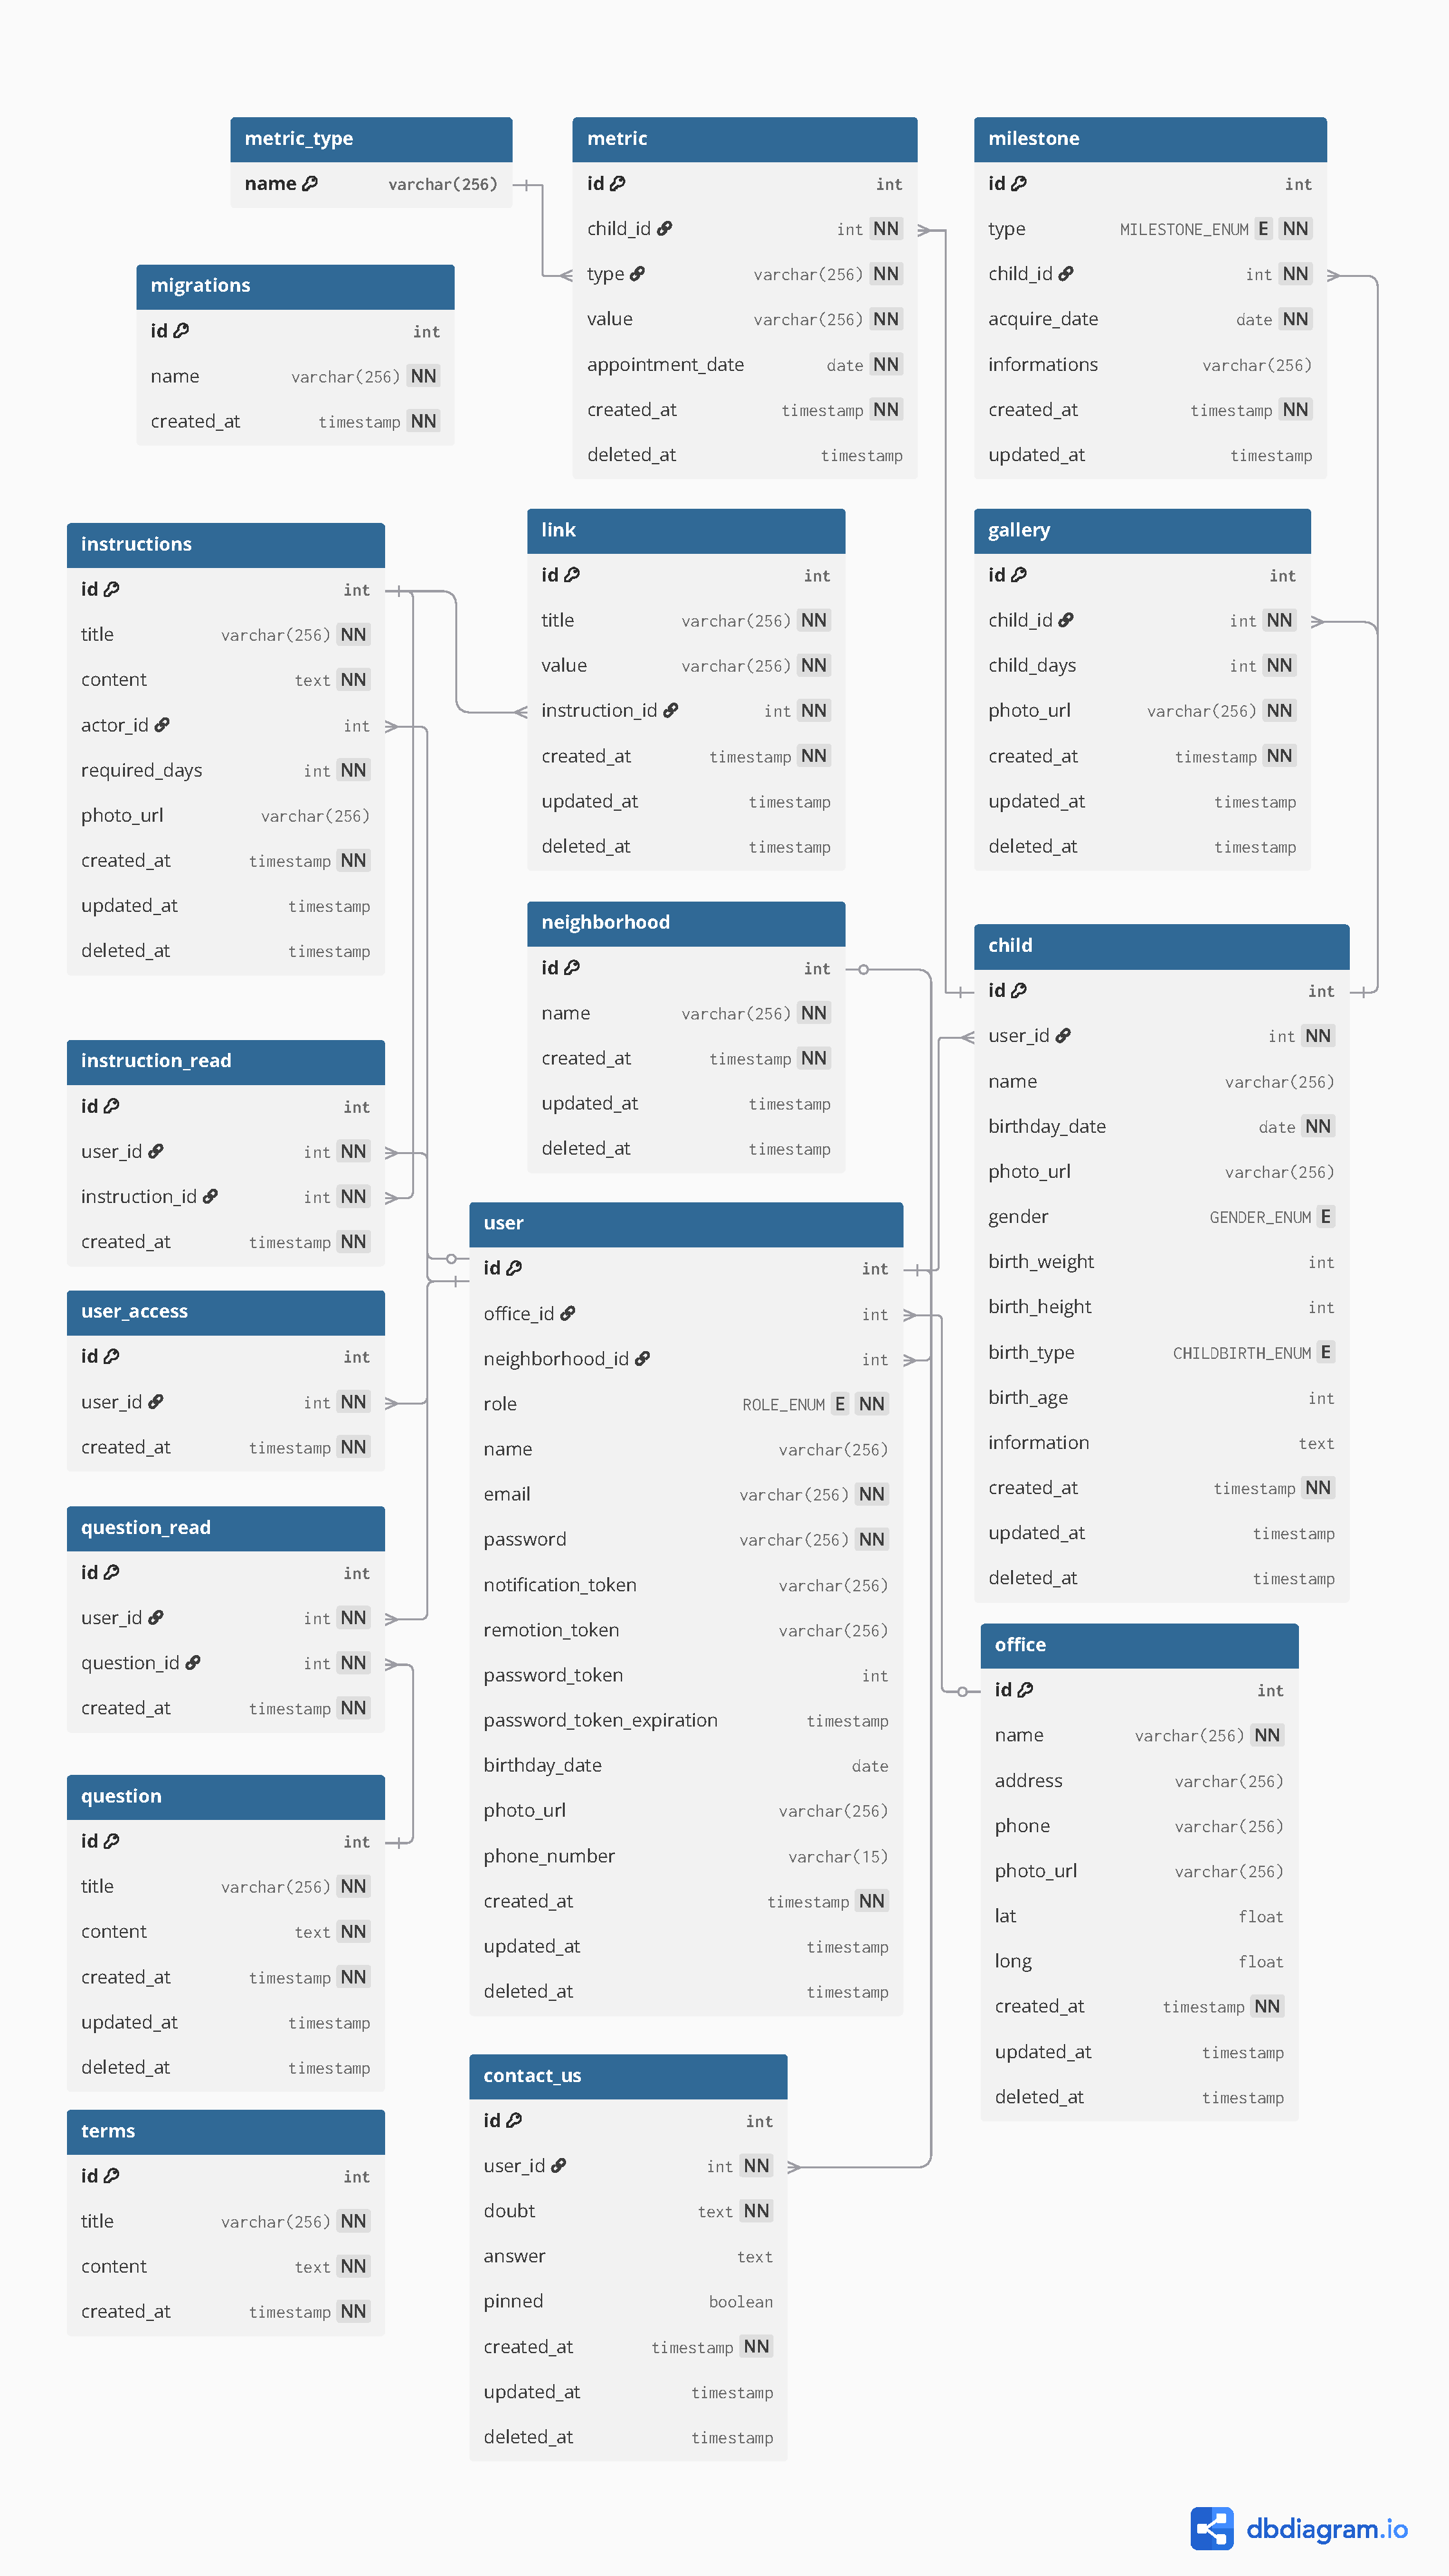
\includegraphics[width=0.85\textwidth]{imagens/modelogic4.pdf}
    \caption{Modelo Lógico do Banco de Dados do Pró-Mamá}
    \label{fig:modelo_logico}
    \legend{Fonte: Elaborado pelo autor (2025).}
\end{figure}

Com o modelo lógico definido, procedeu-se à geração do modelo físico no PostgreSQL. Foram criadas as tabelas, os índices e os relacionamentos conforme especificado, utilizando os recursos nativos do sistema gerenciador de banco de dados \cite{postgresdocs}.

\subsection{Configuração do ambiente}

% Descrever a configuração do ambiente de desenvolvimento local
% Como o painel e api usam node, foi configurado o nvm para gerenciar as versões do node
% Foi feita a instalação do docker e docker compose para facilitar o desenvolvimento e implantação
% Os recursos da API foram instalados via Docker com um arquivo compose configurado no repositório
% O painel usa ReactJs e foi configurado o ambiente com create-react-app Typescript do Vite

A configuração do ambiente de desenvolvimento local buscou padronizar as ferramentas utilizadas pela equipe e simplificar a replicação do sistema. Considerando que tanto a \emph{API} quanto o Painel Administrativo utilizam \emph{Node.js}, optou-se pela instalação do \emph{NVM} (\emph{Node Version Manager}) para gerenciar as versões da plataforma de execução.

Para facilitar o desenvolvimento e a implantação dos serviços, foi adotado o \emph{Docker} em conjunto com o \emph{Docker Compose}. Essa escolha permitiu encapsular os recursos da \emph{API}, como banco de dados PostgreSQL e cache Redis, em contêineres configurados por meio de um arquivo \emph{compose} presente no repositório \cite{dockerdocs}.

O Painel Administrativo foi desenvolvido com \emph{React.js} e \emph{TypeScript}, utilizando o \emph{Vite} como ferramenta de construção e servidor de desenvolvimento \cite{vite}. Essa configuração proporcionou tempos de compilação reduzidos e suporte nativo à tipagem estática, contribuindo para maior produtividade e qualidade do código.


\subsubsection{Sistema de arquivos}

% Foi optado por manter a estrutura de arquivos do sistema antigo, usando o próprio servidor para armazenar os arquivos de mídia (imagens) enviados pelos administradores via painel.
% A estrutura de pastas foi mantida, apenas foi feito o espelhamento no Docker da pasta com a API, pois ela quem serve os arquivos via URL

Optou-se por manter a estrutura de armazenamento de arquivos adotada no sistema anterior. Os arquivos de mídia, como imagens enviadas pelos administradores via Painel, permanecem armazenados no próprio servidor de aplicação.

A organização das pastas foi preservada, sendo realizado apenas o espelhamento do diretório de arquivos no contêiner \emph{Docker} da \emph{API}. Essa abordagem garante que os arquivos sejam servidos por meio de URLs geradas pelo \emph{back-end}, mantendo compatibilidade com o aplicativo móvel e simplificando a migração dos dados existentes.

\subsection{Migração}

% Processo de migração dos dados do banco de dados e arquivos do sistema antigo para o novo sistema

\subsection{Desenvolvimento da API}

% Principais funcionalidades: autenticação, autorização, documentação automática com Swagger, upload de arquivos, job de envio de notificações push
\subsection{Protótipo telas}

% Desenho das telas do sistema com Figma e comparação com o sistema antigo.

\subsection{Desenvolvimento do front-end}

% Padrão de desenvolvimento com componentes reutilizáveis, serviços para comunicação com a API, roteamento, formulários, validações, autenticação, autorização.

\subsection{Testes}

% Estratégias de testes unitários e integração na API e testes manuais no front-end. Validação de testes na PR via GitHub Actions.

\subsection{Implantação}

% Criação de repositório de infraestrutura como código com Docker e Docker Compose, configuração de servidor NGINX com HTTPS, deploy contínuo com GitHub Actions. Deploy em servidor ubuntu, Cloudflare, registro de domínio.
